\documentclass{article}
\usepackage{tikz} 
\usepackage[utf8]{inputenc}
\usepackage{amsmath}
\usepackage{listings}
\usepackage{amsfonts}
\usepackage{amssymb}
\usepackage{tabularx}
\usepackage{enumitem}
\usepackage{algorithm}% http://ctan.org/pkg/algorithm
\usepackage[noend]{algpseudocode}% http://ctan.org/pkg/algorithmicx
\usepackage[margin=0.7in]{geometry}
\usepackage{tikz}

\usepackage{graphicx}
\usetikzlibrary{arrows,positioning} 
\usepackage{subcaption}
\thispagestyle{empty}
\usepackage{multicol,caption}
\pgfarrowsdeclarecombine{ring}{ring}{}{}{o}{o}

\DeclareMathOperator{\ringarrow}{\raisebox{0.5ex}{\tikz[baseline]{\draw[ring->](0,0)--(2em,0);}}}

\tikzset{
    %Define standard arrow tip
    >=stealth',
    %Define style for boxes
    observed/.style={
           circle,
           rounded corners,
           draw=black, thick,
           minimum width=2.2em,
           minimum height=2.2em,
           font=\footnotesize,
           text centered,
           },
     latent/.style={
           circle,
           rounded corners,
           draw=black, thick, dashed,
           minimum width=2.2em,
           minimum height=2.2em,
           font=\footnotesize,
           text centered,
           fill=black!10!white
           },
    % Define arrow style
    pil/.style={
           o->,
           thick,
           shorten <=2pt,
           shorten >=2pt,},
    sh/.style={ shade, shading=axis, left color=red, right color=green,
    shading angle=45 }
    
}
   
\begin{document}
\def\ci{\perp\!\!\!\perp} % from Wikipedia


\begin{figure}
\caption{A simple causal graphical model and corresponding action space}
\label{fig:unify_frameworks}
\centering
\begin{subfigure}[c]{0.25\textwidth}
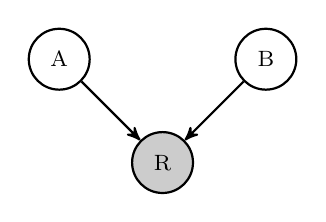
\begin{tikzpicture}[->,shorten >=0pt,shorten <=0pt,node distance=3em,thick,main node/.style={observed}, lt/.style={latent}]
\node[main node](1){A};
\node[main node,fill=black!20!white, below right=of 1](2){R};
\node[main node, above right=of 2](3){B};
\path[]
	(1) edge (2)
	(3) edge (2);
\end{tikzpicture}
\end{subfigure}
\begin{subfigure}[t]{0.4\textwidth}
Actions = \begin{tabular}{|c|}
	\hline
  do(A=0,B=0) \\
  do(A=0,B=1) \\
  do(A=1,B=0) \\
  do(A=1,B=1) \\
  \hline
  do(A=0) \\
  do(A=1) \\
  do(B=0) \\
  do(B=1) \\
  do() \\
  \hline
\end{tabular}
\end{subfigure}
\end{figure}





\begin{equation}
\begin{aligned}
P(R|do(A=1)) & = P(R|A=1) \\
			 & = P(R|A=1,do(B=0))P(B=0)+ P(R|A=1,do(B=1))P(B=1)
\end{aligned}
\end{equation}




\end{document}
